% A good introduction to latex can be found here:
%    http://www.cse.ohio-state.edu/~hank/latex/lshort141.pdf

\documentclass{article}

\usepackage{full page}  % make the margins somewhat smaller than the default

\usepackage{listings}  %  needed for source code listings
\usepackage{color}
\definecolor{dkgreen}{rgb}{0,0.6,0}
\definecolor{gray}{rgb}{0.5,0.5,0.5}
\definecolor{mauve}{rgb}{0.58,0,0.82}

\lstset{frame=tb,
  language=Java,
  aboveskip=3mm,
  belowskip=3mm,
  showstringspaces=false,
  columns=flexible,
  basicstyle={\small\ttfamily},
  numbers=left,
  numberstyle=\tiny\color{gray},
  keywordstyle=\color{blue},
  commentstyle=\color{dkgreen},
  stringstyle=\color{mauve},
  breaklines=true,
  breakatwhitespace=true
  tabsize=3
} 

\usepackage{graphicx}        

% set the document title, author, and date here.
%  once set, the \maketitle command (within the document)
%  will display them nicely
\title{Dartmouth Campus Tour Design Document}
\author{Tianlong Yun, Xiaohong Qiu, Mengjia Kong}

\begin{document}
\maketitle

\section{Introduction}

We are going to make a Dartmouth Guide app. We've found that although similar apps exist, they are not working very well, such as this \"Dartmouth College\" in Play Store. We think app is too simple, a lot of buttons are just link to webpage. What's worse, the map can not even be zoom and move. Besides, the route provided by google map is not cost-aware as it doesn't take the cost totally consumed into account.

We are going make a better one! to make it much easier and more convenient for tourists to explore the campus!

The idea of our app is pretty simple: provide a better interface for Dartmouth tourist, visitors and prospective student. To better achieve our goals, we've identified several features, which is important but can not be found in existing tour guide apps. Furthermore, modern smart phone have a rich set of sensors but existing app don't make use of them, include user-generated content, routing planning and context based notification. 

On the other hand, we are also asking ourselves, what is things that a tour guide person can do but a tour guide app cannot. If the app cannot, is it really cannot? Or we can actually make it happen?

\section{Client}

\subsection{Client Front End}

\subsubsection{Database TableSchema}

The database can be defined as follow:

\begin{lstlisting}
CREATE TABLE IF NOT EXISTS PLACES (
        _id INTEGER PRIMARY KEY AUTOINCREMENT, 
        name TEXT NOT NULL, 
        lat FLOAT NOT NULL, 
        lng FLOAT NOT NULL, 
        pic BLOB, 
        ranking INTEGER, 
        desc TEXT, 
        is_bus_stop INTEGER,
  bus_schedule TEXT
        is_notification_on INTEGER,
  notification_text TEXT,
  notification_voice BLOB);
\end{lstlisting}

Lat and lng are coordinates values. We use BLOB to store the picture representing that place. Ranking ranges from 1 to 5 (with 5 the highest). Is\_bus\_stop determines if there’s a bus stop within 100 meters nearby. Is\_notication\_on means if a voice / text notification should pop out once tourist arrives at this place. We also use BLOB to store the notification if the type is voice-based.

Implement database operations:
\begin{lstlisting}
    // Constructor  
    public PlacesDbHelper(Context context) {
        super(context, DATABASE_NAME, null, DATABASE_VERSION);
    }
    // Create table schema if not exists    
    @Override
    public void onCreate(SQLiteDatabase db) {
        db.execSQL(CREATE_TABLE_ENTRIES);
    }
    // Insert a item given each column value
    public long insertPlace(Place place) {
    }
    // Query a specific place by its index.
    public Place fetchPlaceByIndex(long rowId) {
    }
    // Query the entire table, return all places
    public ArrayList<Place> fetchPlaces() {
    }
\end{lstlisting}

\subsubsection{ListFragment}
ListFragment shows the list of all the recorded places, which is shown in Figure \ref{F:app}.

\begin{figure}[h!]   
\centering
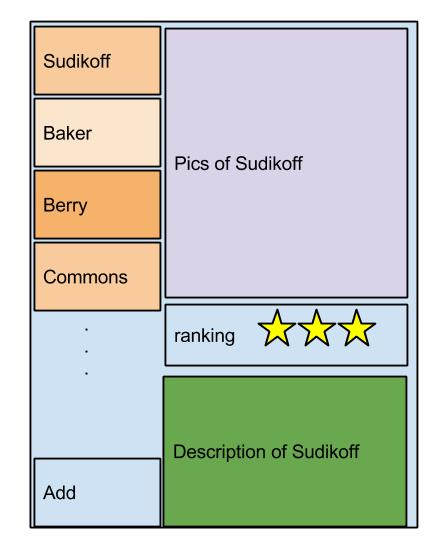
\includegraphics[width = 200pt]{figures/app_interface.jpg}
\caption{Abstract App Interface}
\label{F:app}
\end{figure}

The left hand is a name list of all the places. Once a certain item is selected, it will retrieve picture, ranking and description from database related to that place and displays them according to above order. Since this is community-based tour app, all the data in the database is contributed from tourists. Therefore a button “Add” is added at bottom left. If the place being visited is not in the database and users think others might be interested, just add it into database. While doing adding a place, user has the option to take a picture representing the place, record a live audio as voice notification. Lat and lng can be obtained based on GPS. We use google bus api to determine if there’s any bus stop nearby and acquire bus schedule if yes. If user doesn’t provide a ranking for this place, a default ranking will be applied.

\subsection{Client Back End}

Besides our community-based functions, which allow users to add their own description, pictures and even audio of a place. Our app will also have two very convenient and innovative functionalities. These functions are mostly implemented in the MapActivity.

\subsubsection{Context-aware Notifications}
First, the context-aware notifications, we treat the GPS location information as the “context”. Two kinds of action should happen when user approach some specific location: if it is an attraction, a real tour guide person will be able to start telling a variety of stuff about the location, e.g. history, interesting stories, famous person related to this building. The framework of this service is shown in Figure \ref{F:notifysys}.

\begin{figure}[h!]   
\centering
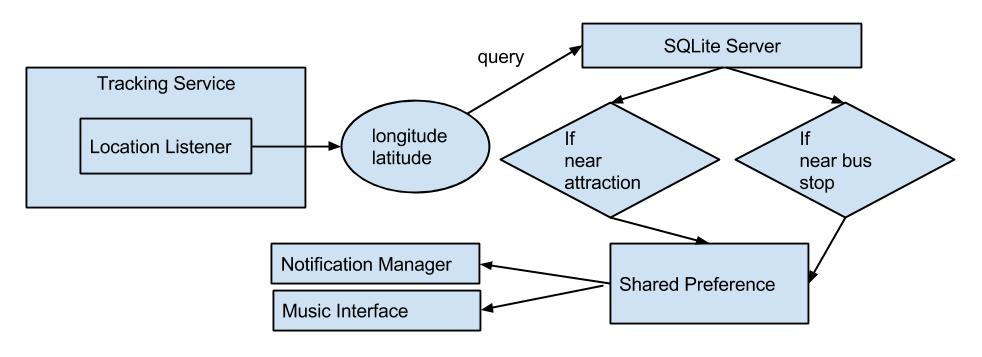
\includegraphics[width = \textwidth]{figures/NotificationGraph.jpg}
\caption{Notification subSystem}
\label{F:notifysys}
\end{figure}


The tracking service is constantly working, retrieving location information (basically longitude an latitude), then the MapActivity will query the SQL server to find out if user is near a location, then based on the user’s preference, appropriate notification will be played, including sound, music and text. The idea here is that user generated content can be also enabled to play in the configuration, so you may see something like this, so current student could generate their own content to show the school, such as Figure \ref{F:fig1}.

\begin{figure}[h!]   
\centering
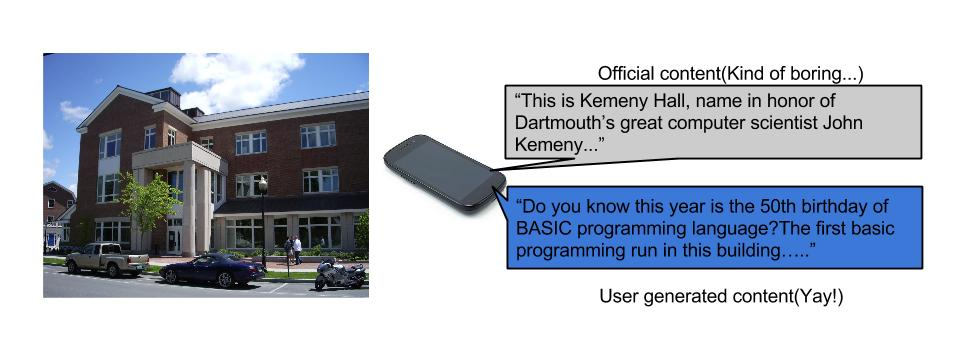
\includegraphics[width = \textwidth]{figures/Fig1.jpg}
\caption{An example of photo which current student show the school}
\label{F:fig1}
\end{figure}


\subsubsection{Bus Notification}
For the bus notification, we will use Google’s bus planning API, once we are near a bus stop, we will call the API and remind the user of upcoming bus. 
The other biggest component is the automatic route planning, for this component, we are considering two kinds of algorithm: A* and Dijkstra’s algorithm. This search can be easily done using Dijkstra’s algorithm. Although an A* algorithm is faster for finding the shortest path between two points, it is not so quick when several target points are given, because it must iterate pairwise searches. As the number of target points increases, the number of duplicated calculations for road network nodes also increases. This duplication degrades efficiency.

So we are going to combine A* algorithm with clustering\cite{htoo2012}, basically, because out campus is a relative small area, several places we are going to visit are actually near each other. So we can do clustering first to reduce the number of source and destination, and then feed the result nodes to our algorithm. Depend on how many nodes and clusters we get, we can even use exhaustion to find the best route. The Figure \ref{F:rpalgorithm} describs the algorithm.

\begin{figure}[h!]   
\centering
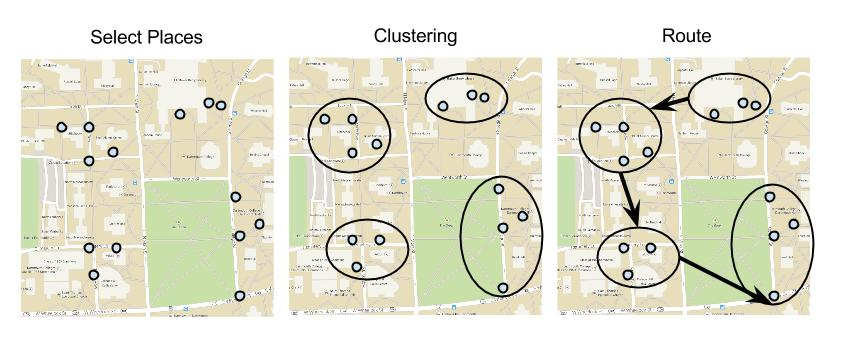
\includegraphics[width = \textwidth]{figures/Clustering.jpg}
\caption{Route Planning Algorithm}
\label{F:rpalgorithm}
\end{figure}

The graph of the MapActivity runs this algorithm, which is shown in Figure \ref{F:algo}.

\begin{figure}[h!]   
\centering
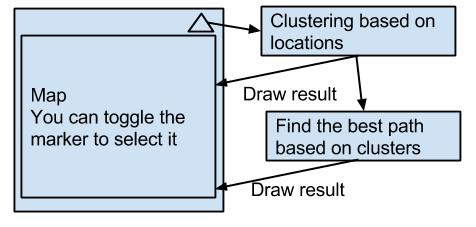
\includegraphics[width = 300pt]{figures/Algo.jpg}
\caption{Route Planning Flow Diagram}
\label{F:algo}
\end{figure}

The structure of the MainActivity is:
\begin{itemize}
\item
BroadcastReceiver for the location information

\item
SQLServer manipulating the Data

\item
Notification Manager

\item
AsyncTask to compute the best route

\end{itemize}


\section{Server}
We design a server which can be controlled both remotely on the cloud and locally on the phone. 

\subsection{Web Interface}

The web interface is in Figure \ref{F:dcserver}. It’s just a sketch. We will improve it according to some cases we run into in the implementation progress.

\begin{figure}[h!]   
\centering
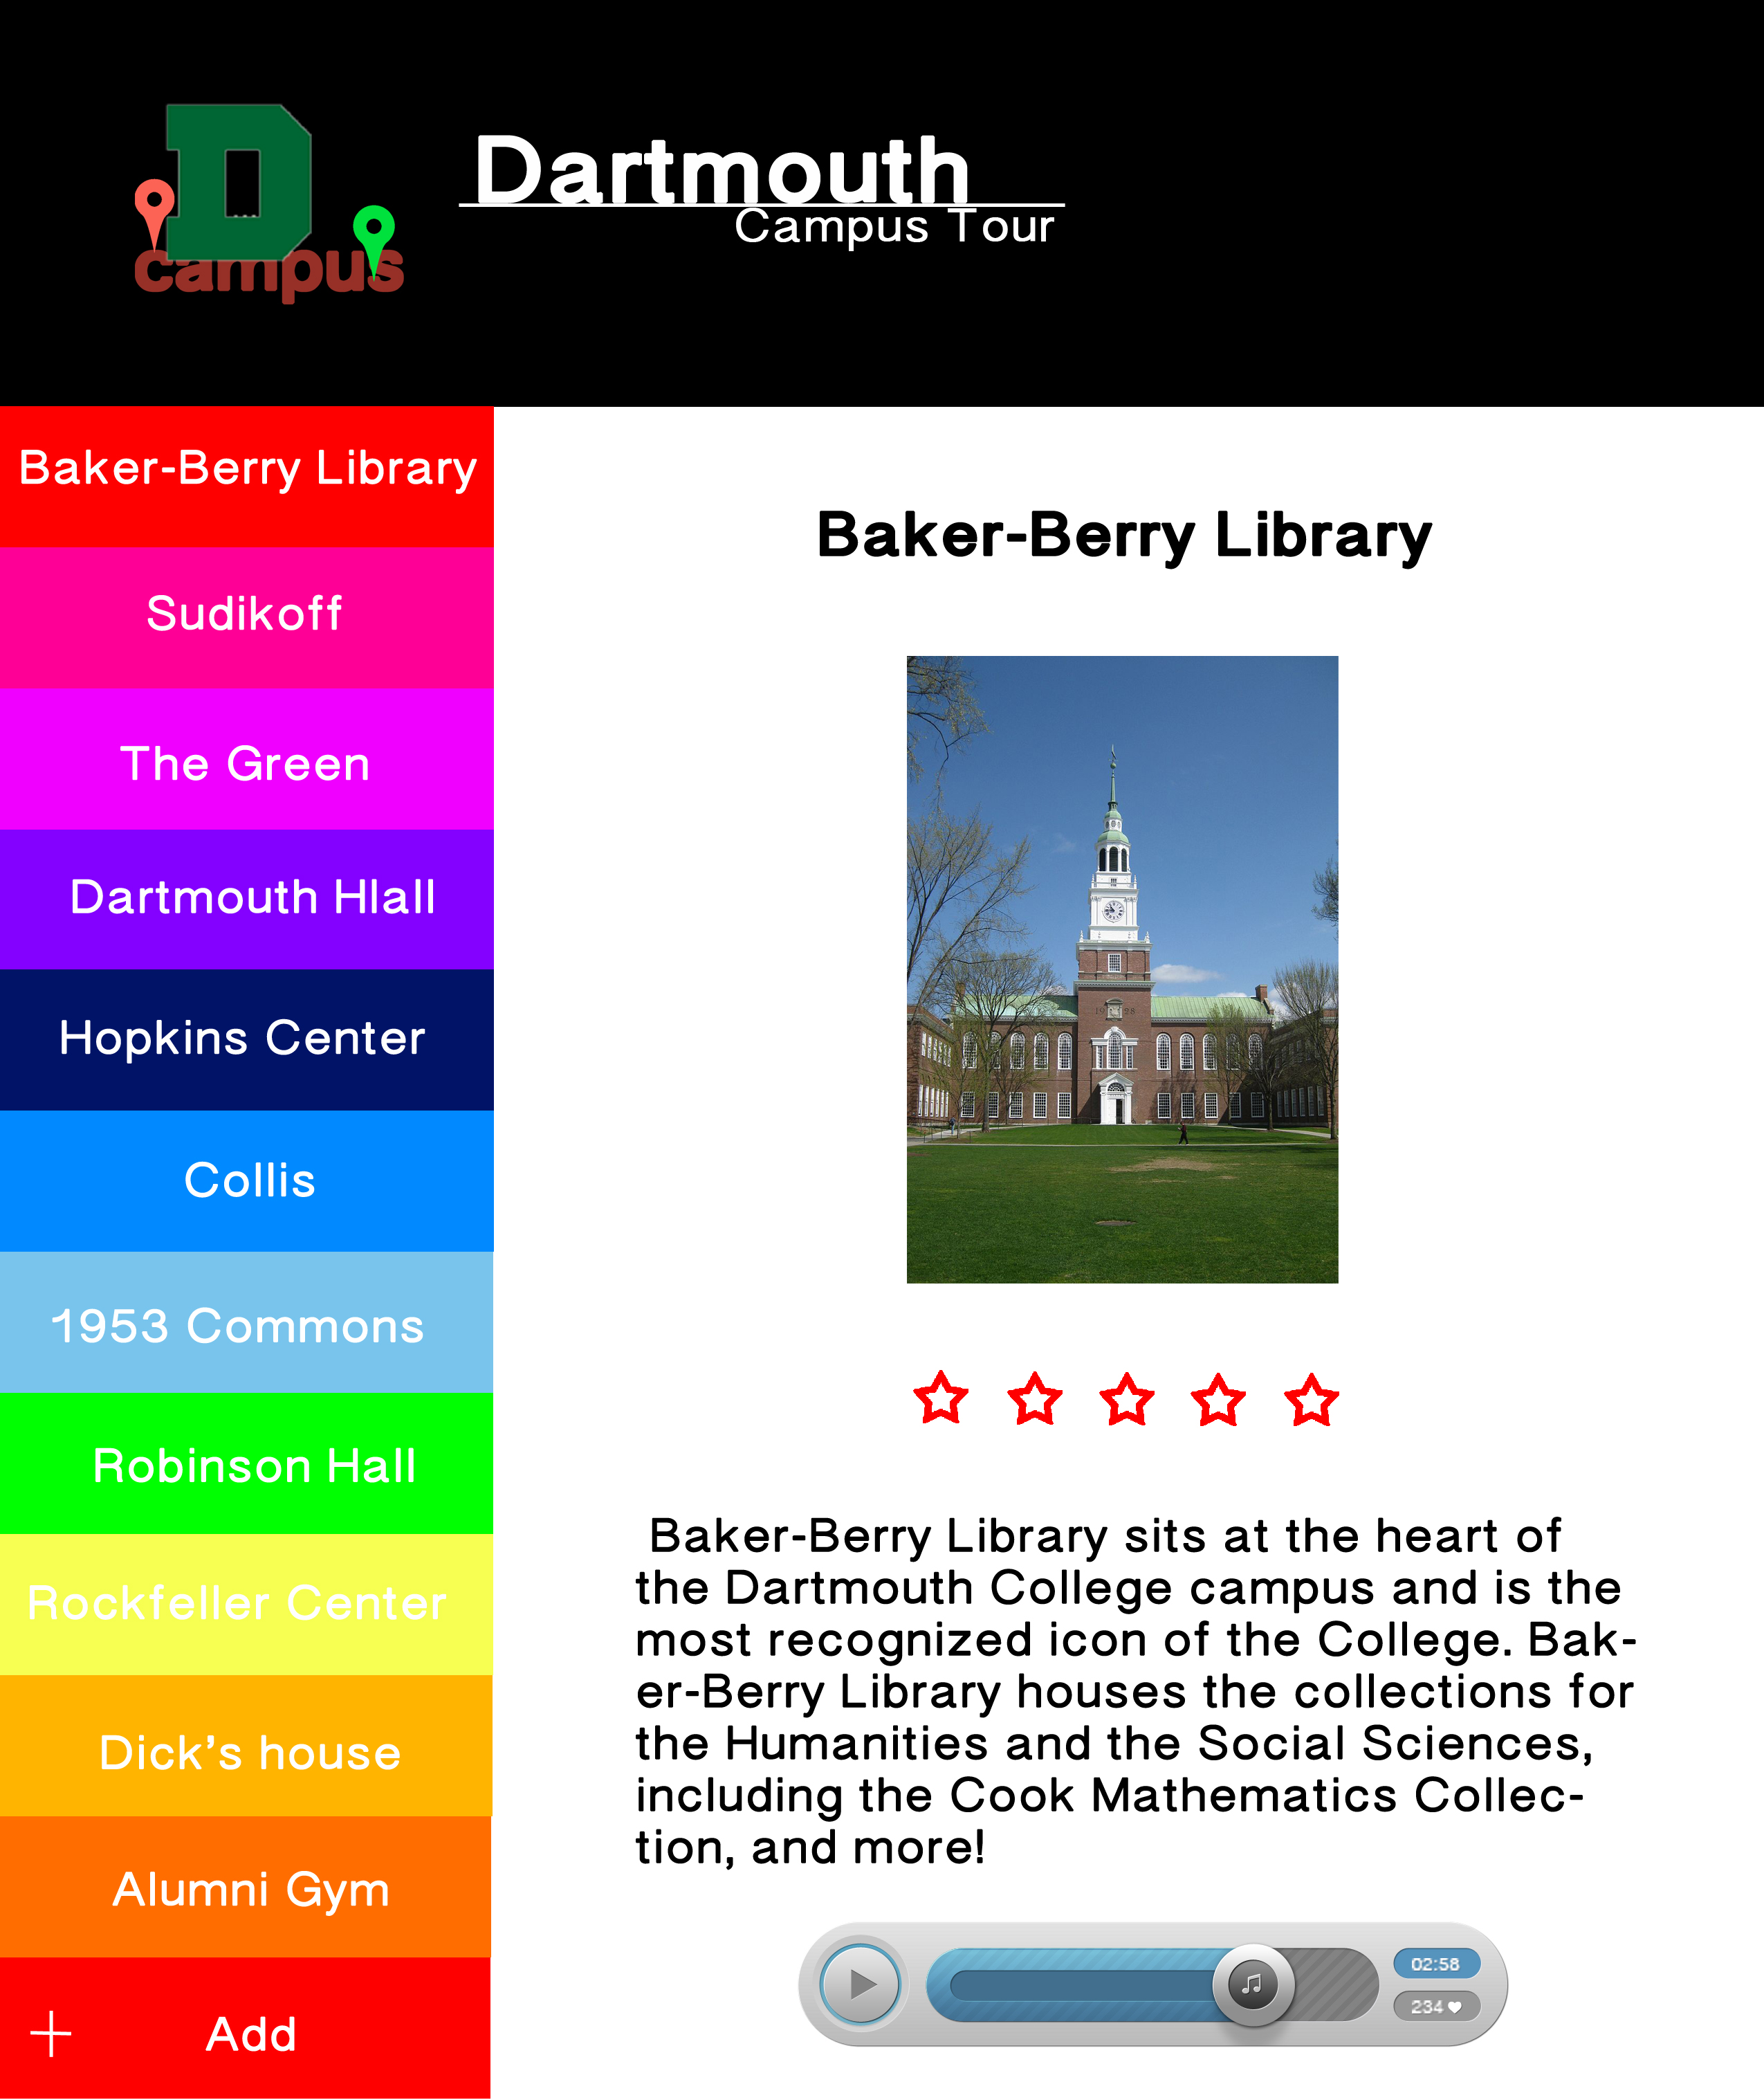
\includegraphics[width = 250pt]{figures/DCampusTourServer.jpg}
\caption{Web interface}
\label{F:dcserver}
\end{figure}

\subsection{Controlled by Server}
There are four functions in server:
\begin{itemize}
\item
Display all locations and details in the web browser. There is a list in the left side which shows all locations’ names. Users can choose one item to show the details in the right side. The details include name, picture, rank, introduction.

\item
Add a location. Click the add button, there will be a form in the right side. Users need to provide the name of the new location, a photo,  a paragraph of introduction of this location and pin the location in the given map. Users also can choose to upload an audio about the location. When the new location to be stored in the server, server will give the location a rank according to data mining all existed locations.

\item
Delete a location. Click the delete button, the entry of this location will be deleted in the server. 

\item
Update information about a location. Click the update button, there will be a form in the right side, which is similar to the add page. Users can modify the name of the location, change a photo, modify the introduction, or upload another audio to cover the old one.
\end{itemize}

Whatever users add, delete or update the information of a location. Server will send a message to any devices to notify them to add, delete or update the entry.

\subsection{Controlled by Client}
The client can add and delete locations as well. When the client add a location, the new entry will be uploaded to Google App Engine. Then users can refresh the browser to see the new entry displayed in the browser. When the client delete a location, the request will be posted to SendDeleteMessageServlet where a message will be sent to all devices and the selected entry will be deleted from the datastore.

\begin{figure}[h!]   
\centering
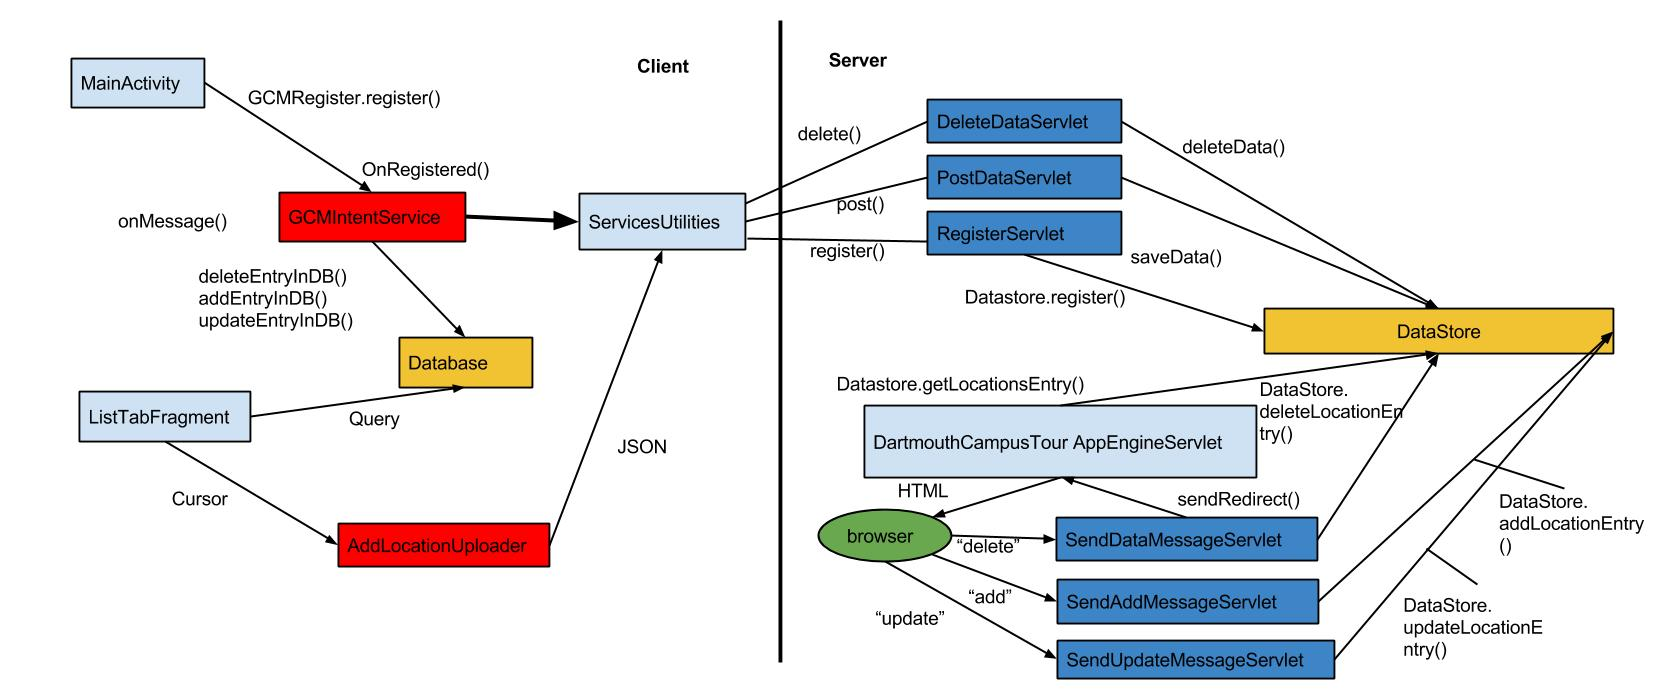
\includegraphics[width = \textwidth]{figures/AppEngineSystem.jpg}
\caption{App Engine System with GCM}
\label{F:appenginesys}
\end{figure}

The Figure \ref{F:appenginesys} shows how clients and server communicates. The app registers Google Cloud Messaging (GCM) in the MainActivity to receive entry deletion updates from the server. When the app is registered with GCM, it sends its device id to the server. The ServerUtilities uses the register() method to send the device id to server’s RegisterServlet. On the server side, RegisterServlet saves the device id into datastore as device entry. The device id is user’s identity. Once user clicked sync, the StartTabFragment retrieves all the entries from the database, then convert them into JSON format. ServerUtilities then posts the JSON format data to server’s PostDataServlet which in turn save the data to the datastore. Note: every exercise entry should have device entry as their parent entity to ensure strong consistency.


\begin{thebibliography}{99}
 \bibitem{htoo2012} Htoo, Htoo, Yutaka Ohsawa, and Noboru Sonehara. \"Single-source multi-target A* algorithm for POI queries on road network.\" Web-Age Information Management. Springer Berlin Heidelberg, 2012. 51-62.


\end{thebibliography}
\end{document}